\documentclass[finalversion]{usetex-v1}
%\usepackage[top=1in, bottom=1in, left=1.25in, right=1.25in]{geometry}
\usepackage[usenames]{xcolor}
\usepackage[colorlinks,linkcolor=red,anchorcolor=blue,citecolor=green,urlcolor=black]{hyperref}
\usepackage{epsfig}
\usepackage{sansmath}
%\usepackage{listings}
\usepackage[]{algorithm2e}
%\lstset{language=C}
%\usepackage{breakurl}
%% Define a new 'leo' style for the package that will use a smaller font.
%\makeatletter
%\def\url@leostyle{%
%  \@ifundefined{selectfont}{\def\UrlFont{\sf}}{\def\UrlFont{\small\ttfamily}}}
%\makeatother
%% Now actually use the newly defined style.
%\urlstyle{leo}
%\linespread{1.2}
%\setlength{\parskip}{1ex}
 
\usepackage{subfigure}
%\usepackage{graphicx}
\usepackage{siunitx}
\usepackage{tikz}
\usetikzlibrary{calc}
\usepackage{pgfplots}
\pgfplotsset{compat=1.8}
\DeclareGraphicsExtensions{.pdf}
\graphicspath{ {./images/}{./figures/} }


%pgfplots setup
\usetikzlibrary{patterns}
\tikzset{ %I believe this sets the defaults, but I am not sure
    hatch distance/.store in=\hatchdistance,
    hatch distance=10pt,
    hatch thickness/.store in=\hatchthickness,
    hatch thickness=2pt
}
\pgfplotsset{
    %You are supposed to use append style rather than just setting
    %parameters globally so they are easier to override to special cases
    %thickness options:thin,ultra thin,very thin,semithick,thick,very thick
    every axis/.append style={
        very thick,
        tick style={thick},
        tick label style={font=\small\mathversion{sans}\sffamily},
        label style={font=\small\sffamily},
        font={\small\sffamily},
        %mark size=1.0
    },
    every legend/.append style={font={\small\mathversion{sans}\sffamily}}
}
\pgfplotsset{
        every mark/.append style={solid}
}

%this is my preferred default cycle list for pgfplots.
\pgfplotscreateplotcyclelist{mcolor}{%
    {blue,every mark/.append style={fill=blue},mark=*},
    {red,every mark/.append style={fill=red},mark=square*},
    {brown,every mark/.append style={fill=brown},mark=triangle*,mark size=3},
    {black,every mark/.append style={fill=black},mark=diamond*,mark size=3},
    {green!60!black,every mark/.append style={fill=green!60!black},mark=pentagon*,mark size=2.5},
    {magenta!90!black,every mark/.append style={fill=magenta!90!black},mark=star,mark size=3},
    {densely dashed,blue,every mark/.append style={fill=blue},mark=*},
    {densely dashed,red,every mark/.append style={fill=red},mark=square*},
    {densely dashed,brown,every mark/.append style={fill=brown},mark=triangle*,mark size=2.7},
    {densely dashed,black,every mark/.append style={fill=black},mark=diamond*,mark size=2.7},
    {densely dashed,green!60!black,every mark/.append style={fill=green!60!black},mark=pentagon*,mark size=2.5},
    {densely dashed,magenta!90!black,every mark/.append style={fill=magenta!90!black},mark=star,mark size=3}}

%uses just line styles instead of marks to differentiate
\pgfplotscreateplotcyclelist{mline}{
    {solid,blue,every mark/.append style={fill=blue}},
    {densely dashed,red,every mark/.append style={fill=red}},
    {densely dotted,brown,every mark/.append style={fill=brown}},
    {loosely dotted,black,every mark/.append style={fill=black}},
    {loosely dashed,green!60!black,every mark/.append style={fill=green!60!black}},
    {densely dashdotted,magenta!90!black,every mark/.append style={fill=magenta!90!black}},
    {densely dashdotdotted,teal,every mark/.append style={fill=teal}},
    {loosely dashdotted,orange,every mark/.append style={fill=orange}},
    {loosely dashdotdotted,violet,every mark/.append style={fill=violet}}}

%fill pattern for bar charts similar to the gnuplot one used previously
\pgfplotscreateplotcyclelist{mfill}{
    {fill=white,postaction={pattern=crosshatch,pattern color=red}},
    {fill=white,postaction={pattern=north east lines,pattern color=green}},
    {fill=white,postaction={pattern=north west lines,pattern color=blue}}}

    \pgfplotsset{cycle list name=mcolor}


\newcommand{\comments}[1]{}
\newcommand{\todo}[1]{\textit{\color{red}#1}}

\begin{document}
%\title{Selective Deduplication for VM Snapshots in Cloud Storage}
%\title{ Low-Cost Data Deduplication  for  Virtual Machine Backup in Cloud Storage}
\title{Parallel Deduplication with Batch  Scheduling for  Collocated Virtual Machine Backup in the Cloud}
%\title{Data Deduplication and Zipf-like Distribution in VM Cloud Storage}

\author{
Daniel Agun$^{\star}$,  
Wei Zhang$^{\star}$, and Tao Yang$^\star$ \\
{\normalsize$^\star$  University of California at Santa Barbara} 
%{\normalsize$^\dagger$Alibaba Inc.}
%Wei Zhang, Tao Yang, Gautham Narayanasamy\\
%University of California at Santa Barbara
%\and
%Hong Tang\\
%Alibaba Inc.
}

% \{wei, tyang\}@cs.ucsb.edu

\date{}
\maketitle

%need to explain: vm cloud, vm backup, dedup fundamentals, vm dedup(2 works), distributed dedup, zipf
%need to define: requirements, design considerations, architecture

\begin{abstract}
Backup in VM cloud is mainly done by storing snapshots of
VM images. Since VM images are huge and backup is frequent, 
the snapshot storage
in VM cloud must reduce snapshot data to save cloud resources.
Thus it is very important to exploit the duplication pattern of snapshot
backup data for developing better cloud storage system.
In this paper we present the data duplication pattern that
we observed from Aliyun's publie VM cloud services, and provide
some insights for researchers and engineers to design future
 deduplication strategies for VM cloud backup.
\end{abstract}
\section{Introduction}
In a virtualized cloud environment such as ones provided by Amazon EC2 and Aliyun,
each instance of a guest operating system runs on a virtual machine, accessing
virtual hard disks represented as virtual disk image files in the host operating system.
Because these image files are stored as regular files from the external point of view,
backing up VM's data is mainly done by taking snapshots of virtual disk images.

Frequent  backup of VM snapshots increases  the reliability of VM's hosted in a cloud.
For example, Aliyun, the largest cloud service provider by Alibaba in China, 
provides automatic frequent backup of VM images to strengthen the reliability of its service for all users.
The cost of frequent backup of VM snapshots is  high because of the huge storage demand.

Unlike the legacy backup systems\cite{jumbo07} dealing with general file-level backup and deduplication, 
Backing up VM images is different: although each VM image is treated as a file logically from
external point of view, its size is very large.
On the other hand, a cloud must support parallel backup of a large number of virtual disks everyday. 
Two key requirements we face during desinging a backup storage system for VM snapshot are: 
\begin{enumerate}
\item VM snapshot backup should only use a minimal amount of system
resources so that most of resources is kept for regular cloud system services and VM themselves.
\item The entire snapshot storage and deduplication process must be fully decentralized to acheive
high scalibility and throughput, 
no component shall become a bottleneck.
\end{enumerate}

It is impossible to accomplish such requirements without fully utilizing the data duplication pattern
in VM snapshot backups
and design the optimal data deduplication strategies.
Thus we believe the first step towarding a cost-effective deduplication solution
 is to exploit the characteristics and duplication pattern of VM snapshot data. 

There are several previous studies on this topic. Jayaram\cite{Jayaram2011} and
Jin\cite{Jin2009} has investigated the data similarity between VM images using 
Rabin's fingerprinting\cite{identify00} algorithm. 
Silo\cite{xia2011} and Extreme Binning\cite{extreme_binning09} studied the problem
of deduplication in a large distributed environment which also helps solving the
problem of VM snapshot backup.

In this paper we present the data analysis of Aliyun's VM snapshot data,
our focus is to find out exploitable data duplication patterns and
correspoding factors.
Our work differs from previous studies at several aspects:
First, we are targeting at the problem of snapshot backups, 
and no previous study has studied VM image with backup data involved.
Second, we focus on observing the pattern of data duplication in VM snapshot backups,
rather than examining the effect of variable-sized chunking algorithm.
Finally, we use real user's VM data rather than hand-made VM images.

The rest of the paper is organized as follows: Section~\ref{sect:setup} introduces
the experiment setups, Section~\ref{sect:dedup} studies the potential of deduplication
in VM snapshot backups, Section~\ref{sect:loc} discusses the locality factor
in reduction of backup data,
Section~\ref{sect:scale} analysis the change of data duplication against system scale,
Section~\ref{sect:dup} introduces the patterns of heavily duplicated data.

\section{Experiment Setup}
\label{sect:setup}
We sampled two data sets from Aliyun's public VM cluster, where all VMs
are used by real world users running various applications such like
database, web server, rendering services or even Hadoop. Each VM has
two virtual disks, one is for OS and software installations, and the other one
is for storing user data contents.

Data set VOSS composes of the OS disks from 35 VMs in 7 popular OSes: 
Debian, Ubuntu, Redhat, CentOS, Win2003 32bit, win2003 64 bit and win2008 64 bit. For each OS, 
5 VMs are chosen, and every VM come with 10 full snapshots of it OS disk. So
there is 350 full snapshot backups in this data set, the overall size is about 7 TB.
We use VOSS to study the backup duplication characteristics and OS disk change patterns.

Data set DDS contains the first snapshots of 1323 VMs' data disks from a cluster with 100+ nodes. 
Since no backup duplication is involved in this data set, this data set helps us to 
study the duplication pattern of user generated data. The overall size of DDS is near 23 TB. %introduce the vm cloud, backup problem, and our requirements

\section{Background and Related Work}
\label{sect:background}


At a cloud cluster node providing access to multiple virtual machines, each
instance of a guest operating system runs on a virtual machine (VM), accessing
virtual hard disks represented as virtual disk image files in the host
operating system. For VM snapshot backups, file-level semantics are normally
not provided, and snapshot operations take place at the virtual device driver
level.  This meands no fine-grained file system metadata can be used to
determine the changed data.

Another issue is the sheer size of the backups. to maintain mutiple daily
uncompressed snapshots of each VM would be very expensive, even though
most of the data remains the same from day to day, and even between VMs common
software packages and operating systems mean that the amount of unique data is
much smaller. Backup systems have been developed to use content fingerprints to
identify duplicate content~\cite{venti02,Rhea2008}. Offline deduplication is
used in~\cite{EMC,NetAppOffline} to remove previously written duplicate blocks
during idle time.  Several techniques have been proposed to speedup searching
of duplicate fingerprints. For example, the data domain method
~\cite{bottleneck08} uses  an in-memory Bloom filter and a prefetching cache
for data blocks  which may be accessed.  An improvement to this work with
parallelization is in ~\cite{MAD210,DEBAR}.  As discussed in
Section~\ref{sect:intro}, there is no dedicated resource for deduplication in
our targeted setting and low memory usage is required so that the resource
impact to other cloud services is minimized. Approximation techniques which
reduce the memory requirement at the expense of deduplication efficiency are
studied in~\cite{extreme_binning09,Guo2011,WeiZhangIEEE}.  In comparison, this
paper focuses on full deduplication without approximation

%%In a virtualized cloud environment such as ones provided by Amazon EC2\cite{AmazonEC2} and Alibaba Aliyun\cite{Aliyun}, 
%At a cloud cluster node, each instance of a guest operating system runs on a virtual machine, accessing virtual hard disks 
%represented as virtual disk image files in the host operating system.
%For VM snapshot backup, file-level semantics are normally not provided.
%Snapshot operations take place at the virtual device driver level, which means no fine-grained file system metadata can be used to determine the changed data. 
%%Only raw access information at disk block level are provided. 
%%Each physical machine hosts many VMs and petabytes of data in a cloud cluster need a frequent  backup. 
%%Ideally speaking, snapshot backup must not affect the normal cloud service, which means that 
%%only a very small slice of cluster resource can be used for the backup purpose.



%%The previous work for storage backup has extensively used  data deduplication techniques can eliminate redundancy globally among different files from different users.
%Backup systems have been developed to use content fingerprints to identify duplicate
%content~\cite{venti02,Rhea2008}.
%Offline deduplication is 
%used in ~\cite{EMC,NetAppOffline} to remove previously written duplicate blocks during idle time.
%%,NGmiddleware2011}.
%%Today's commercial data backup systems (e.g. from EMC and NetApp)
%%\cite{emc_avamar}\cite{datadomain_whitepaper}
%%use a variable-size chunking algorithm to detect duplicates in file data~\cite{similar94,hydrastor09}.
%Several techniques have been proposed to speedup searching of duplicate
%fingerprints. For example, the data domain method ~\cite{bottleneck08} 
%uses  an in-memory Bloom filter and a prefetching cache for data blocks  which may be
%accessed.  An improvement to this work with parallelization is in ~\cite{MAD210,DEBAR}.
%As discussed in Section~\ref{sect:intro},
%there is no dedicated resource for deduplication in our targeted setting and low memory usage
% is required so that the resource impact to other cloud services is minimized.
%%NG et al.~\cite{ NGmiddleware2011}  use
%%a related filtering technique for integrating deduplication in Linux  file system and the memory
%%consumed is up to 2GB for a single machine. That is still too big in our context discussed below.
%%Lillibridge et al.~\cite{sparseindex09} break list of chunks
%%into large segments, the chunk IDs in each incoming segment are sampled and the segment is
%%deduplicated by comparing with the chunk IDs of only a few carefully selected backed up segments.
%%These are segments that share many chunk IDs with the incoming segment with high probability.
%The approximation techniques are studied in~\cite{extreme_binning09,Guo2011,WeiZhangIEEE}  
%%Deepavali et al.~\cite{extreme_binning09} and Zhang et al.~\cite{WeiZhangIEEE}  
%to reduce memory requirement with a tradeoff of the reduced deduplication ratio.
%%use fingerprint-based file similarity  and group similar files into the same physical location (bins) to deduplicate against each other.
%%That leads  to a smaller amount of memory usage for storing meta data in fingerprint
%%lookup  
%In comparison, this paper focuses on  full deduplication without approximation.
%%We also take advantages of the fact that in a VM cloud environment,
%%the virtual device driver can easily keep track if  large data
%%segments have been modified using dirty bits and such information can avoid sending
%%unmodified data segments for deduplication, which significantly saves cost.



Additional inline deduplication techniques are studied in ~\cite{sparseindex09,Guo2011,idedup}. 
All of the above approaches have focused on
such inline duplicate detection in which  deduplication of an individual block  is on the critical write path.
In our work, this constraint is relaxed and 
there is a waiting time for many duplicate detection requests. This relaxation is acceptable because 
in our context, efficiently finishing the backup of VM images within a reasonable time window is more
important than optimizing individual VM block  backup requests, and by batch
processing the deduplication requests we can decrease resource usage.




\comments{
This paper considers a backup service uses the existing cluster computing resource. 
Another option is to attach  a separate backup system with deduplication
support the cluster, and  every machine can periodically transfer snapshots to
the attached backup system.
%One  weakness of this approach is communication bottleneck between a large number of machines
%in a cloud to this centralized  service.
The cost of allocating the above dedicated backup  resource can be expensive.
Since most of backup data is not used eventually, CPU and memory resource in such a backup service may 
not be fully utilized. This paper seeks for a low-cost architecture option.
}
%It should be emphasized that our approach does not  accumulate raw backup data temporarily for deduplication
%and does not require a significant amount of extra storage capacity.
%Our strategy is to perform a drity  scan to collect
% a small amount of disk space  to accumulate
%deduplicate requests along with necessary meta data, and perform actual backup after deduplicate detection completes.
  
%affecting the overall time of backup. 
 %related works, related solutions, 
\section{Design Overview}
%[describe what is going to be presented in this section]
We start by analyzing the main features in the design of our system.
We first present its architecture,
then introduce the two major contributions: the colocated deduplication 
scheme and the snapshot deletion strategy.
\subsection{Architecture}
%[describe the cloud environment]
Our architecture, as shown in figure.\ref{fig:arch}, is built on top of 
Alibaba's platform which is the largest cloud service provider in China. 
A typical VM cluster in our cloud environment
consists of from hundreds to thousands of physical machines, each of which can
host tens of xen-based\cite{Barham2003} VMs.
Alibaba's cloud platform provides a hadoop-like infrastructure, 
which includes several highly scalable distributed service:
\begin{description}
\item[Distributed file system] This is a scalable distributed file system (DFS) being optimized for many large and sequential reads or appends. DFS holds the responsibility of managing physical disk storage
in the cloud. All data needed for VM services, such as virtual disk images used by runtime VMs,
and snapshot data for backup purposes, reside in this distributed file system. 
%\item[KV]: a distributed key-value store for managing structured data.
%\item[MapReduce]: a distributed data processing framework supports Map-Reduce\cite{Dean2004}.
\item[Distributed memory cache]: A distributed memory object caching system helps us to hold the fingerprints of those popular data blocks for deduplication inqueries. 
\end{description}
In addition, our implementation also uses MapReduce to facilitate the offline
data processing, and stores a small amount of snapshot metadata in a 
BigTable-like persistent key-value store. 

%[describe the benefits of using mature cloud technologies]
In general, our snapshot system and the virtual machine management service 
rely on these fundamental cloud services
to be functional. Such a colocated deduplication architecture allow us 
to enjoy the benefits from these mature technologies 
such as load balancing, scalability, and fault tolerancy.
Moreover, all the above cloud services can easily find their open-source counterparts,
which improves the generality of our architecture and deduplication scheme.

{\bf Snapshot Representation}
The virtual device driver uses a bitmap to track the changes 
that have been made to virtual disk.
Every bit in the bitmap represents a fix-sized (2MB) region called \textit{segment}, indicates whether the segment
is modified since last backup. Hence we could treat segment as the basic unit 
in snapshot backup similar to
file in normal backup: a snapshot could share a segment with previous snapshot it is not changed. 
Moreover, we break 
segments into var-sized chunks (average 4KB) using content-based chunking algorithm,
which brings the opportunity of fine-grained deduplication by
allowing data sharing between segments.

\begin{figure}[htbp]
  \centering
  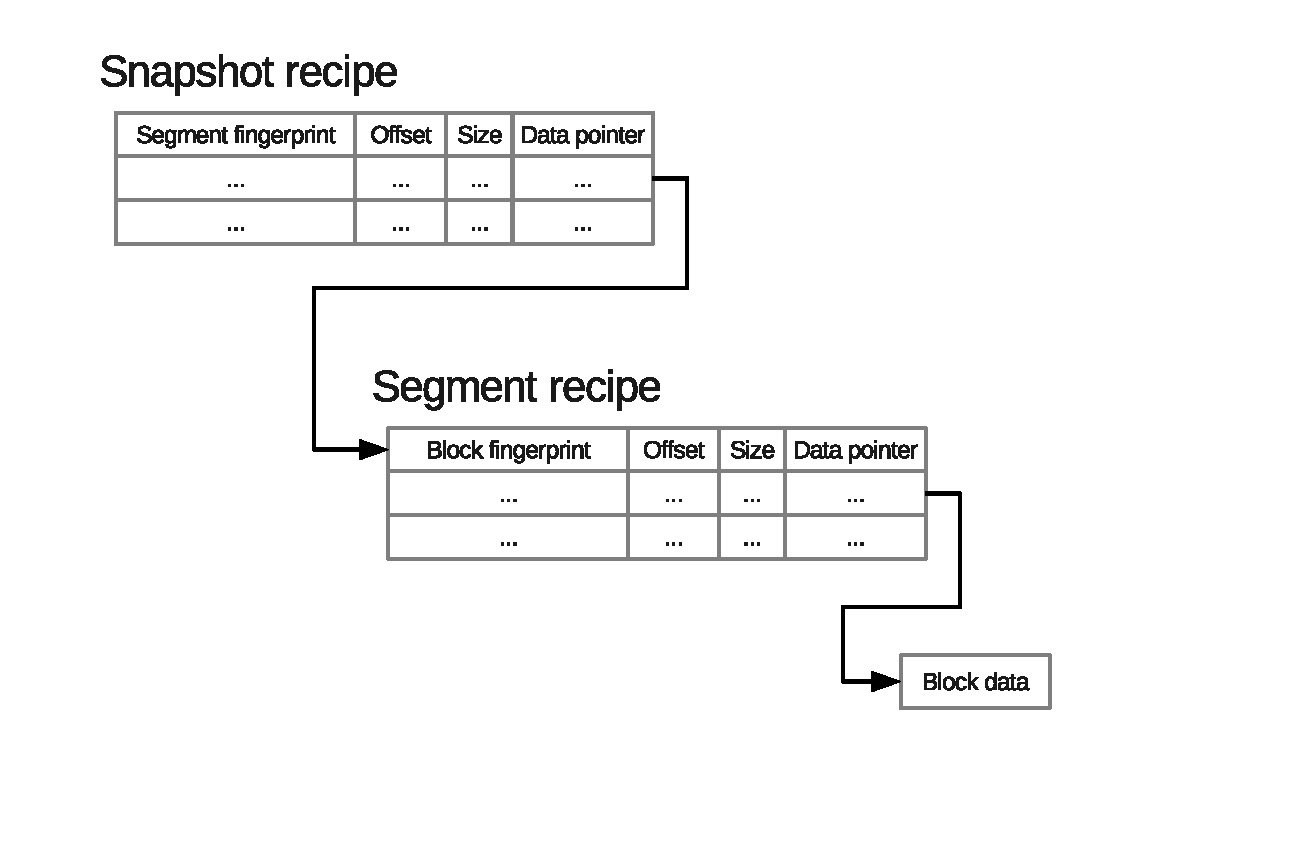
\epsfig{file=images/snapshot_representation.pdf, width=3.7in}
  \caption{An example of snapshot representation.}
  \label{fig:snapshot_rep}
\end{figure}
As a result, the representation of each snapshot is designed as a two-level index data structure 
in the form of a hierarchical directed acyclic graph as shown in Figure \ref{fig:snapshot_rep}.
A snapshot recipe contains a list of segments, each of which is represented as a segment recipe
that holds the meatdata of its chunks. We choose this two-level structure because in practice we
observe that during each backup period only a small amount of VM data are added or modified. 
As the result, even the metadata of two snapshots can be highly similar, 
thus aggregating a large number of chunks as one segment can significantly reduce the space cost of snapshot metadata.
Furthermore, instead of using variables-sized segments, we use a dirty bit to capture the change status of fix-sized
segments which greatly ease the segment-level deduplication.

In both two kind of recipes, 
they do not include the actual data but only have
 references point to the data which are either stored in append store or CDS.
In our implementation the data reference is a 8 bytes field which is either an 
ASID (discuss in \ref{sect:append}) or an offset of an additional flag indicates
the location of CDS data.

\begin{figure}
    \centering
    \subfigure[Node architecture from VM point of view]
    {
        \includegraphics[width=3in]{images/socc_arch_vm.pdf}
        \label{fig:arch_vm}
    }
    \\
    \subfigure[Cluster architecture]
    {
        \includegraphics[width=3in]{images/socc_arch_cluster.pdf}
        \label{fig:arch_cluster}
    }
    \caption{System architecture}
    \label{fig:arch}
\end{figure}

%[describe the architecture frm node side]
{\bf Node Architecuture} 
Our node-side architecture, depicted in figure.\ref{fig:arch_vm}, consists of
two main entities: a virtual block device driver, and a snapshot deduplication component.

%[brief the virtual device driver]
One physical node hosts tens of VMs, each of which access its virtual machine disk image through the
virtual block device driver (called TapDisk\cite{Warfield2005} in Xen).
This driver maintains a map of dirty-bits to record
the change status of every fix-size segment of the virtual disk. 
When the VM issue a disk write, the bits coresponding to the segments that covers 
the modified disk region are set, thus letting snapshot deduplication component knows these
segments must be checked during snapshot backup. After the snapshot backup is finished, 
snapshot deduplication component acknowledges the driver to resume the dirty-bits map to
a clean state.

%[brief the snapshot deduplication]
The snapshot deduplication component consists of the chunking and deduplication 
logic of our snapshot storage system. We choose 

It contains an append store client which provides facilities to manage stored snapshot data, and a CDS client to support CDS index access. We will further discuss our deduplication scheme in section\ref{sec:dedup}.

%[describe the arch from cluster side]
{\bf Cluster Architecture}

%[describe the data structure in underlying storage]
{\bf Append Store}
Append Store (AS) is our underlining storage engine for storing snapshot data after deduplication. 
AS is built on top of our highly scalable distributed file system (DFS), 
which is very similar to Google's file system
in a sense that it is optimized for large files and sequential read/append operations.

\begin{figure}[htbp]
  \centering
  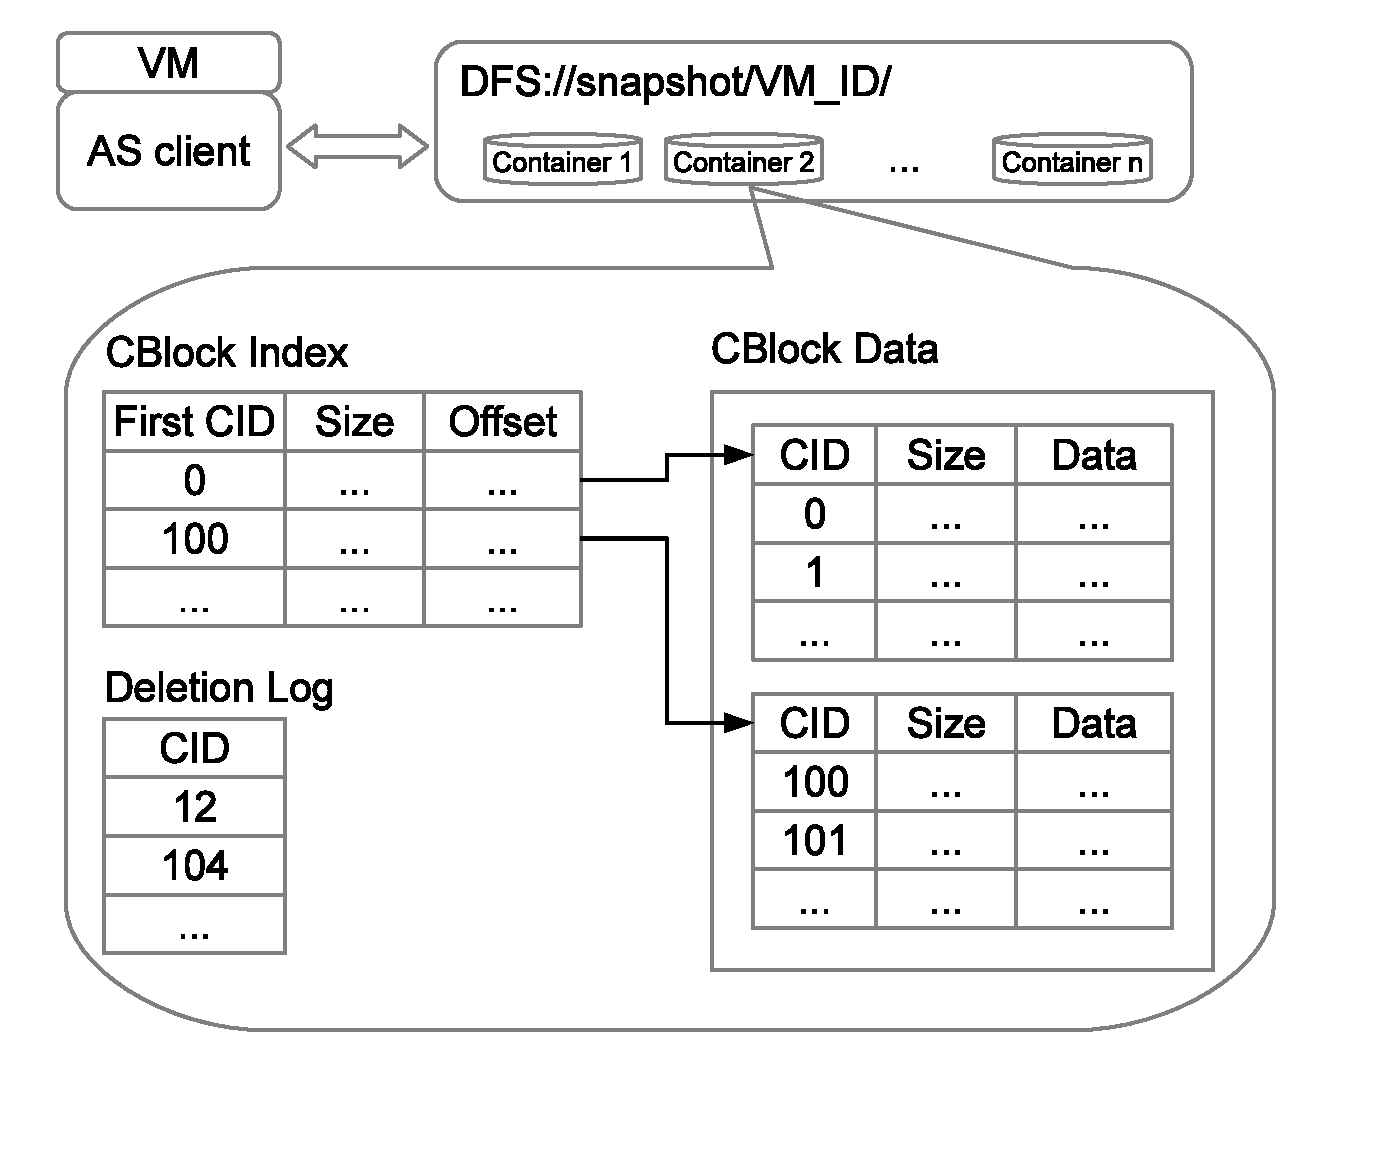
\epsfig{file=images/append_store_arch.pdf, width=3.5in}
  \caption{Architecture of Append Store}
  \label{fig:as_arch}
\end{figure}

Append Store supplies three interfaces: {\em get(ref)} accepts a data reference and retrives data, 
{\em put(data)} accepts data and returns a reference to be stored in metadata recipes, 
{\em delete(ref)} 
deletes the data pointed by the reference.
Under the hood, small var-sized data are grouped and stored into larger data containers. Each VM has
its snapshot data stored in its own Append Store, specified by the VM ID. 
We split every Append Store into multiple data containers so that reclaiming the disk space would not 
result in rewriting all the data at the same time.

As shown in Fig.\ref{fig:as_arch}, every data container is represented as three data files in DFS:
the data file holds all the actual data, the index file is responsible for translating data reference
into data locations, and a deletion log file remembers all the deletion requests to the container.

A data reference is composed of two parts: a container ID (2 bytes) and CID (6 bytes).
Append Store assign every piece of data a CID for its internal data referencing. 
When new data is appended, its CID is the current largest CID in that container plus one.
As a result, all the data locations are naturally indexed by this self-incremental CID, 
no extra sorting is needed.

Append Store groups multiple chunk data (i.e., 100) into larger units, called {\em CBlock}.
CBlock is the basic unit for append store's internal read/write/compression.
There is one index entry in the container index corresponding to every CBlock. It keeps the first chunk's CID
in that CBlock, and the CBlock data's size and location.

Using CBlock brings us several advantages: First, the write workload to DFS master is greatly reduced; second, grouping
small chunks gives better compression. Third, reading a CBlock (200 - 600 KB) typically cost the same amount of disk 
seek as reading a 4KB chunk. Finally, this greatly reduces the size of index. Let $m$ be the number of chunks in each
CBlock, then the overall index size is reduced to $1/m$. In our implementation, using $m=100$ reduces the index for
a 1GB container from 10 MB to 100 KB.

In order to read a chunk data by reference, Append Store client first loads the
container index file specified by the container ID, then search the CBlock index to find the entry that covers the chunk by CID.
After that, it reads the whole CBlock data from DFS, decompress it, seek the exact chunk data specified by CID. 
Finally, the client updates itws internal chunk data cache with the newly loaded contents to anticipate future sequential reads.

Write requests to append store are accumlated. When the number reaches $m$, the AS client forms a CBlock by assigning 
every chunk a CID, compress the CBlock data, and append it to the CBlock data file. Then a new CBlock index entry is appended
to CBlock index.

Append store adopts lazy delete strategy. The deletion requests are appended into every container's deletion log file with the CID of data to be deleted.
CIDs in deletion log are guaranteed to be referenced by nobody and can be safe deleted in future. 
Periodically, snapshot management system asks append store to compact containers in order to reclaim disk space. 
The actual compaction will only take place when the number of deleted items reached $d\%$ of container's capacity. 
During compaction, append store creates a new container (with the same container ID) to replace the 
existing one. This is done by sequentially scan the old container, copying all the chunks that are not 
found in deletion log to the new container, creating new CBlocks and indices. 
However, every chunk's CID is plainly copied rather than re-generated. This does not affect the sorted
order of CIDs in new container, but just leaving holes in CID values. As the result, all data references stored 
in upper level recipes are unaffected, and the data reading process is as efficient as before.

\subsection{Snapshot Deduplication and Fault Isolation}
\label{sect:dedupe}
%snapshot representation
%\subsection{Inner and corss VM deduplication}
Our  deduplication scheme compares the fingerprints of the current snapshot
with its parent snapshot and also other snapshots in the entire cloud.
This process performs   the duplication in two categories: \textit{Inner-VM} and \textit{Cross-VM}. 
Inner-VM duplication exists between VM's snapshots, because the majority of data are unchanged during each backup period. 
Such localization increases data independency between different VM backups,
simplifies snapshot management and statistics collection,
and facilitates parallel execution of snapshot operations.
On the other hand, Cross-VM duplication is mainly due to widely-used software and libraries. 
As the result, different VMs tend to backup large amount of highly similar data.
Our multi-level pipeline process can minimize 
the cost of deduplication while maximize the its efficiency at each level,
and it is parallel since each segment is processed independently.

\begin{itemize}
\item \textbf{Dirty-based corase-grain inner-VM deduplication.}
The first-level deduplication is to follow the standand dirty bit approach, but is conducted
in the coarse grain segment level.
We use the  Xen virtual device driver which supports dirty bits for thestorage device
and the dirty bit setting is maintained in a corase grain level we call it a segment.
In our implementation, the segment size is 2MB. 
Since every write for a block will touch a dirty bit, the device driver maintains dirtybits in memory
and cannot affort a small segment  size.

\item \textbf{Chunk-level fine-grain nearby duplicate detection.}

The best deduplication uses a nonuniform chunk size 
in the average of 4K or 8K~\cite{??}.
Thus the second-level inner-VM deduplication is to assess in this
level, but only for those dirty  segments. 
We load the fingerprints of block chunks of the corresponding segment from the
parent for a comparisons and compare near-by fingerprint matching within this segement.
The amount of memory for maintaining those fingerprints  is small.
For example, with a 2MB segment, there are about 500 fingerprints to compare.


%If we use 4KB in level-1, then such a level-1 should have similar dedup efficiency 
%as the current level-1 and level-2 combined, because finally they equal to comparing  
%parent snapshot at 4KB granularity.
%
%However, at level-3 things are different. If we use 4KB fix-size block uniformly, it would be harder for different VM to share data through CDS, because there is no guarantee that the location of duplicate data on different VM disks are always aligned at 4KB boundary. For example, if two VMs each has a copy of duplicate data, but they are not aligned, then we won't be able to detect them. Our study at the current small data set has shown that using 4KB fix-size block will make CDS method less efficient by nearly 10%. Over the long time, more and more OS variations will co-exist in the cluster, making this 4KB fix-size approach inefficient in reducing duplicate data across VMs.

%\item \textit{Level 2  Chunk fingerprint comparison.}
%If a segment is modified, we perform fine-grained deduplication 
%by comparing the fingerprints of its chunks to the same segment's recipe in the previous snapshot,
%thus eliminate partial data duplication within the segment.
%\end{itemize}
%
%In general, operations at level 1 have almost no cost and most of unmodified data are filtered here. 
%To process a dirty segment at level 2, 
%there requires no more than one DFS access to load the segment recipe from previous snapshot,
%and a tiny amount of memory to hold it in main memory.

\item \textbf{Cross-VM deduplication.}
This step accomplishes the standand global fingerprint  comparison as conducted
in the previous work~\cite{??}.
One key observation is that the inner deduplication has removed many of duplicates.
There are not lot of deduplication opportunities cross VMs while the memory
consumption for global comparison is expensive.
Thus our approximation is that duplicate sharing patterns among  VM follows
a zip-like distribution, and the global fingerprint  comparison  only searches
for the most popular items. 
\end{itemize}

{\bf Popular Chunk Management and VM-oriented Fault Isolation}
Our objective for fault isolation is to minimize the number of VMs affected when there are failures
in the cluster.  The inner-VM deduplication does not depend on any global service and the comparison
for each VM is localized within the parent and the current snapshot.
Thus there is no data dependence between VMs.
For cross-VM deduplication, there is a data dependence among VMs and we would minimize the faiulre impact
of shared blocks by adding extra replcas of those shared blocks.

This section analyzes the choice of popular blocks and its impact on the deduplication efficiency.
It also  compares the  fault resilience of our VM-centric deduplication approach with a standand approach using 
global deduplication.


{\bf Impact of CDS deduplication.}
Our empirical study based on VM images from production environment\cite{ieeecloud} showed that the
frequency of data duplication follows Zipf-like distribution\cite{zipf},
with the exponent $\alpha$ between 0.65 ~ 0.70.
As a result, it can be proved that deduplication efficiency of CDS index is scalable:

For the Zipf-like distribution, an approximation to the sum of the first $n$ 
elements of the distribution can be derived as follows:
\begin{equation}
\sum_{i=1}^{n}\frac{1}{i^\alpha}\approx \int_{1}^{n}\frac{1}{x^\alpha}\mathrm{d}x=\frac{x^{1-\alpha}}{1-\alpha}=\frac{n^{1-\alpha}}{1-\alpha}\;  for\;  \alpha<1
\end{equation}

So the cumulative distribution function for a CDS holding top $S_c$ fingerprints
of global index with size $S_g$ is:

\begin{equation}
  E = (S_c / S_g)^{1-\alpha} \;  for\;  \alpha<1
\end{equation}

%[Describe the dedup efficiency model in detail]
Let $N$ be the number of nodes in the cluster, $m$ be the memory on each node that are used by CDS, $D$ be the amount of data on each node, and $B$ be the average block size. Then $S_c$ and $S_g$ can be expressed as:
\begin{equation}
S_c = N*m/F, S_g = N*D/B
\end{equation}

By replacing $S_c$ and $S_g$ in the first formula, the deduplication efficiency becomes:
\begin{equation}
  E = (\frac{m*B}{F*D})^{1-\alpha}
\end{equation}

Since $B$, $D$ and $F$ are pre-configured constants, the deduplication efficiency of CDS is only controlled by the its memory usage.

\subsection{Snapshot Summaries for Deletion} %, design considerations, architecture
%\section{ Performance Analysis and Comparison}
\label{sect:analysis}

We assume a flat architecture that we use all machines in a cluster to host virtual machines, and also evenly host  raw data and meta data of the temporarily accumulated requests.  We call global index to be the meta data of all non-duplicate chunks such as chunk fingerprints and reference pointers.

Following parameters are used to analyze the performance of our system.
\begin{itemize}
\item
$p$ is the number of machines in a cluster. These machines can run in parallel for backup. The request buckets are evenly distributed among these machines.
\item $v$ is the number of virtual machines per machine. At Alibaba, $v=25$.
\item $x$ is the number of snapshots saved for each VM.
\item $k$ is the number of iterations to complete all virtual machine backup. Each iteration performs v/k backups.
\item $t$  is the  amount of temporary disk space used per physical machine for deduplication.
\item $m$ is the amount of memory used per each physical machine for deduplication. Our goal is to minimize 
\item $s$ is the average size of virtual machine image. At Alibaba data we have tested, $s=40GB$.
\item $d_1$  is the average  deduplication ratio using  segment-based dirtbit.  s*d1 represents the amount of data items that are duplicates and can be avoided for backup. For Alabalba dataset tested, 
$d_1$=77\%.
\item $d_2$ is the average  deduplication ratio using content chunk fingerprints after segment-based deduplication. For Alaba dataset tested,  $d_2=50$\%.
\item $b$ is the average disk bandwidth for reading from local storage at each machine. 
\item $q$ is the number of buckets to accumulate requests at each machine. Thus the total number of buckets is $p*q$.
\item $c$ is the chunk block size in bytes.  In practice $c=4KB$.
\item $u$ is the record size of detection request per block.  In practice, 
\item $u$=40. That includes block ID and fingerprint.
\item $m$ is the maximum memory allocated for deduplication purpose.  A $g$ fraction used for 
machine-machine network  request buffering and $(1-g)$ fraction used for memory-disk bucket buffering.
\item $e$ is the size of a duplicate summary record for each chunk block.
\item $\alpha_n$ is the startup cost for sending a message in a cluster. $\alpha_d$ is the startup cost 
such as seek for disk IO. $\beta$ is the time cost for in-memory duplicate comparison.
\end{itemize}
The system keeps at most  $ x$ copies of snapshots for each VM on average.  The total size of  global content fingerprints is $x*s*v/c*u *(1-d1)*(1-d2)$ where $c$ is the average chunk size and $u$ is the meta data size of each chunk fingerprint. In practice $c=4K$ and $u/c$  is about 100.  $x=10$ in the case of Alibaba cloud.

Define $r = s v (1-d_1)/(ck)$  which is the total number of duplicate detection requests issued at each machine and at each iteration.

We first discuss the memory usage and processing time  of 3 steps. 
 For Step 1,  the buffer for sending requests from one machine to another has a size of  $g*m/p$, and with such a buffering, the total number of outgoing communication messages from  each machine to other machines  can be 
\[
r u p/(g*m)
\]
The total  amount of data communicated among machines is relatively small: $r u p$ in the cluster, distributed among $p$ machines.

Once every machine receives detection requests and divide them into buckets, it writes the content to the disk once the buffer is full. The buffer for each bucket is $(1-g)m/q$ and the total number of disk write requests issued after the bucket buffer is full is:
\[
r u q/((1-g)*m)
\]
The total time for step 1  which  reads VM images and write accumulated detection requests  is:   
\[
r  ( c+  u) /b   +r u /m (\alpha_n  p/g  + \alpha_d q/(1-g)  )
\].

For Step 2,  part of memory at each machine is  to hold  a bucket of global index and accumulated requests. That is
\[
m_b= x*r *u*k(1-d_2)/q + r*u/q
\]
Thus the memory requirement for this portion can be made very small when setting a large q. On the other hand, as the system detects duplicates per hash bucket, we need to allocate buffer space for receiving  duplicate summary for each VM.  The total buffer size is $m-m_b$ which is used evenly for $v$ VMs.

The size of  the duplicate summary for each bucket is
\[
S_{sum}= sv(1-d_1)e /(k c q)
\]
We can buffer the outcome of multiple buckets. The total buffer factor is 
\[
(m-m_b)/ S_{sum}.
\]
The final bucket buffer for each VM is still fairly small, and writing such a buffer to the disk may involve two I/O requests (one to fetch the old block, and one is to update). The total seek cost involved 
\[
2*v*\alpha_d*q/ ((m-m_b)/S_{sum})= 2v r e  \alpha_d / (m-m_b)
\]
Thus the total time of Step 2 takes
\[
( x*r *k*u*(1-d_2) + r*u) / b_d  + r* \beta+   2v *r*e \alpha_d /  (m-m_b).
\]


The key cost of step 3  is to read the nonduplicate parts of each VM and output the backend storage. The time of Step 3  takes:
\[
2 r *c* (1-d_2) /b_d
\]
That assumes that when a content chunk is not a duplicate, there is a significant number of non-duplicate  chunks following that  chunk. 

Thus the total time to process all $v$ virtual machines after $k$ iterations are:
\[
k [
r  ( c+  u) /b   +r u /m (\alpha_n  p/g  + \alpha_d q/(1-g)  )
+( x*r *k*u*(1-d_2) + r*u) / b_d  + r* \beta+   2v *r*e \alpha_d /  (m-m_b)
+2 r *c* (1-d_2) /b_d
]
\]
subject to conditions that
\[
m - m_b> 0
\]

The total disk requirement  per machine for hosting the global index  and meta  data of  accumulated requests is:
\[
x*r *k*u*(1-d2) + r*u.
\]
That is not so big, and is acceptable as we show later.




\subsection{A Comparison with Other Approaches}

The memory  space requirement for the data domain approach with bloomer filter is:
\[
x*r k u (1-d2)/r
\]
where $r$ is the bloom filter with about  1:10 ratio in practice.  The disk space used  is 
\[
x*r *k *u*(1-d_2).
\]


 %, design considerations, architecture
\section{Round Scheduling}
\label{sect:scheduling}
The simplest way to take advantage of the efficiency of batch processing is to
schedule all the work to be done in one round.  This works well if all of the
data being backed up are only copies, e.g. a separate backup system which data
is sent to over the network. However, in our case we are backing up the
original virtual disk, which may still be in use during the snapshot. This adds
extra complexity to the cost analysis, because we must now also consider the
cost of maintaining a constistent view during the snapshot process. We use the
Copy on Write (CoW) provided by the virtual disk manager to maintain a
consistent view. With CoW, the
duration of the backup affects how much data must be copied. Other studies have
shown that as much as 8\% or even more of total capacity must be reserved for
CoW \cite{EMCIncrementalDataChanges}. The actual cost of CoW is a factor of the
data size, the write rate, and duration CoW is taking place. The data size
isn't something we can change, nor the write rate, but we can minimize the
duration that a given VM is undergoing CoW. We assume a poisson distribution of
writes (which closely fits the meaured results from
\cite{EMCIncrementalDataChanges}), and then try to minimize the CoW cost using
our performance and CoW model. Although the single batch schedule completes the
backup in the smallest amount of time, it also has the greatest CoW cost
because the most processing must be done before any VM can release the CoW
lock.

Our basic CoW cost model is:
\[
    CoW=n(1-e^{-m/n})
\]
    where
\[
    m=tw(1-d_1)c
\]

In the above model, $n$ is the number of dirty segments, $t$ is the time under
CoW, $w$ is the
write rate during CoW, $d_1$ is the \% of clean data (which doesn't go under
CoW), and $c$ is a constant determining how likely writes are to touch dirty
segments which haven't yet been copied vs. dirty segments which have already
been copied during the current backup. With this CoW cost model and the earlier
performance model, we can estimate the CoW cost of a given backup schedule.
Note that CoW ends in Stage 2b, so only the time up to the end of 2b counts
towards CoW. \todo{we still need to pick a value for $c$}

We can see above that the way to decrease the CoW cost is to decrease t, the
time the virtual disk is under CoW. We do that by breakng up the backup into
multiple
rounds, where in each round the CoW cost is minimized. The more rounds there
are the shorter each round can be and therefore the smaller the CoW cost. The
more rounds there are however the greater the backup overheads and some of the
efficiency gained from batch processing is lessened. We balance these costs by
setting a time limit on the whole backup job, and then develop an algorithm to
schedule VMs into rounds and pick the number of rounds to use.

With these parameters a model that closely fits our goals is the dual version
of the
bin packing problem. In standard bin packing the goal is to fit all of the
items into as few bins as possible, without overfilling any bins. In the dual
version of the problem however as many bins as possible are to filled to at
least some minimum level. This fits our purpose because we want to maximize the
number of rounds, with some constraint to keep the efficiency benefits of batch
processing. In our dual-bin-packing solution the constraint is to keep the total
cost of the schedule under a time limit rather than mandating a minimum bin
level. We
adapt an algorithm for dual bin packing\cite{DualBinPacking} to fit our VM
scheduling problem. The algorithm adapted is called iterated A and works by
iteratively callng a bin packing heuristic A with the items to be scheduled and
the number of bins, using binary search to arrive at the best number of
bins. A(I,N) is defined to return the optimality of packing set I into N bins
using A. We take this basic idea and look at several VM packing heuristics to
arrive at an efficient packing algorithm. More formally, our adaptation of the
iterated A algorithm is defined as:


%lstset{basicstyle=\ttfamily\tiny
%}
\todo{justify choice of initial UB (right now it is mostly arbitrary)}
\begin{lstlisting}
Set UB=min(n,2*v)
Set LB=1
while UB>LB
  set N = (UB+LB+1)/2
  if A(machines,N) > T, set UB=N-1
  else set LB=N
Halt
\end{lstlisting}
where A(machines,N) returns the total backup time of the schedule for N rounds\\
This algorithm returns the packing generated by A(machines,UB) after loop finishes

The general algorithm relies on a good choice of A to arrive at an efficent
packing. Our first VM packing heuristic, A0, is a na\"\i{}ve approach very
close to the un-adapted algorithm from the dual bin packing paper. For both
algorithms we develop, in case of ties, choose the left-most item.

A0:
\begin{lstlisting}
sort VMs in descending order by size
while there is an unscheduled VM
  pick the first unscheduled VM a
    pick the round with the current
    lowest runtime b
  schedule VM a to round b
Halt
\end{lstlisting}

A0 decreases CoW cost (see Table~\ref{tab:schedule-costs}), but has room for
improvement. The first issue is that the round with the current lowest runtime
is chosen.  Because backup time is dependent on a combination of the highest
machine load and average machine load, if we add a VM to the currently most
loaded machine in a round it will increase runtime much more than if we add the
VM to a different round where that machine is currently empty
\todo{(insert figure to show how this happens)}. Therefore a better scheduling
would be obtained if we pick the round with the lowest runtime after we
simulate adding the new VM to that round. This new round picking heuristic
takes into account that the same VM might have different affects on different
rounds. This aspect of round picking must be considered because we assume a VM
must be backed
up by the machine that hosts it. If the VMs are located on a DFS such that they
can be
backed up by any machine in the cluster then the problem of load balancing
becomes a simpler but much different problem, and isn't considered here. We
also pick the most heavily loaded (i.e. most data remaing) machine in case of
ties so we can make the most backup progress in a round.

Another improvement we can make to A0 is to the VM picking heuristic. For the
same reason as given above, the largest VM may not always have the greatest
impact on time (e.g. picking a slightly smaller VM on the most heavily loaded
machine has a greater impact than selecting the largest VM on a lightly loaded
machine). A better way to pick VMs than just by size is to simulate removing
VM's, then model the new single round time, and pick the VM whose removal most
decreases the single round time (i.e. the VM that has the greatest impact on
overall backup time). By picking VMs this way we take into account
the machine load in picking which VM to schedule next, and minimize the time
the remaining VMs will take to backup

After making the two above changes we arrive at VM packing heuristic A1.

A1:
\begin{lstlisting}
while there is an unscheduled VM
  pick the VM a whose removal will
    most decrease single round time
    tie-breaker:VM on most heavily
    loaded round
  pick the round b whose runtime will
    be lowest after adding VM a
  schedule VM a to round b
Halt
\end{lstlisting}

A1 significantly improves our simulated results, bringing our CoW costs much
closer to the best case than the worst case, as can be seen in
Figure~\ref{tab:schedule-costs}.  Our current implementation of the algorithm
focuses on the deduplication and so doesn't make use of CoW, but we can see
that our simulated times closely match measured runtimes (hopefully). \todo{I
haven't actually implemented the schedulers into the dedup yet to test this}
 % CoW cost considerations and round scheduling

\section{Evaluation}
\label{sect:exper}

We have implemented and evaluated a prototype of the partition-based deduplication scheme on a Linux cluster
of AMD Bulldozer FX8120 and Intel Nehalem E5530 machines.  Objectives of our experimental evaluation are:
1) Analyze the processing time and throughput of backup for a large cluster of virtual machines.
2) Assess the effectiveness  of partition-based duplication detection 
backup.  3) Examine the impacts of buffering during meta data exchange.

\subsection{Experimental setup}

Our implementation is based on Alibaba's Xen cloud platform~\cite{Aliyun,WeiZhangIEEE}.  
At Alibaba's Aliyun, the  target is to backup cluster of a few thousands nodes with 25 VMs on each machine.
%We are running our deduplication/backup  service on 100 nodes.
%Memory usage is about 150MB space per node during backup and
%the CPU usage is very small during the experiments. 
Based on the Alibaba data studied,  each VM has about  40GB of storage  data usage on average
including OS and user data disk.  The backup of VM snapshots is completed within a few  hours every night,
%and that translates to an aggregated backup throughput of 139GB per second, or 500TB per hour.
%  For 2 hours, every machine can do 139MB/second. For 3 hours, then 92MB/second
For each VM, the system keeps 10 automatically-backed snapshots in the storage while
a user may instruct extra snapshots to be saved.

% the system must finish saving daily snapshots of all VMs in 2 hours. In our typical 1000 nodes cluster, each node hosts 25 VMs, each VM has 40GB of data on average, that translates to backup throughput of 139GB/second, or 500TB/hour.

%In our snapshot deduplication architecture, CDS is the key to achieve greater deduplication than
%incremental backup solutions. Our basic assumption of CDS us that VM disks, especially OS disks,
%have huge amount of data in common, and such common data can be represented by a relatively smaller data set
%because of their high appearence frequency. As a result, the major portion of snapshot deduplication effect shall 
%emerge from eliminating the duplication of such a small data set. In this section, we evaluate
%the effectiveness of CDS using real user VM disks from our production VM cluster.

%Since it's impossible to perform large scale analysis without affecting the VM performance,
%We have sampled a data set from 1323 real user VMs from a cluster with 100 nodes 
%to measure the effectiveness of our scheme.
We have performed a trace-driven study using a dataset containing 10 snapshots of 35 VMs.
That is part of a 1323 VM dataset  collected from 100 Aliyun's cloud nodes 
in our earlier work with  Alibaba Aliyun~\cite{WeiZhangIEEE}.
%In this dataset, there are 10 snapshots per each VM user and the total amount of space 
%investigated is 17.5 terabytes.
%This dataset contas compose of 35 VMs from 7 popular OSes: 
%Debian, Ubuntu, Redhat, CentOS, Win2003 32bit, win2003 64 bit and win2008 64 bit. For each OS, 
%5 VMs are chosen, and every VM come with 10 full snapshots of it OS and data disk. 
%The overall data size for this 700 full snapshots is 17.6 TB.
%This dataset  contains the snapshots of 1323 VMs.
%Since inner-VM deduplication is not involved in the first snapshot, this data set helps us to 
%study the CDS deduplication against user-related data. The overall size of dataset2 is 23.5 TB.
All data are divided into 2 MB fix-sized segments and each segment is divided into 
variable-sized content blocks ~\cite{similar94,rabin81} with an average size of 4KB.
The signature for variable-sized blocks is computed using their SHA-1 hash. 
%Popularity of data blocks are collected through global counting 
%and the top 1\% will fall into CDS, as discussed in Section~\ref{sect:crossVM}.

\comments{

Each VM file is  divided into content blocks of
variable sizes~\cite{similar94,rabin81} with an average size of 4KB. 
The signature for variable-sized blocks is computed using  their SHA-1 hash. 
Each segment is of size 2MB.  
Popularity is computed by using 90\% of dataset, which reflects our setting that the system recomputes
CDS every 1-2 days to catch up the popularity trend.
}
%seg, and we performed global perfect deduplication 
%to caculate the number of duplicate copies of each individual unique block. We choose 2KB, 4KB, 16KB as the minimum, average
%and maximum block size
%OS data
%user data: zipf
%prediction
%say something about aliyun


%To compare the effectiveness with a full deduplication approach with an approximation,
%we use  extreme binning and perfect deduplication~\cite{extreme_binning09}. 
%For perfect deduplication and extreme binning, each snapshot is also divided into chunk blocks
%using TTTD with an average size of 4KB. The original extreme binning work uses the whole file
%as the input unit and  this size is too big in our system. 
%Thus we split each image snapshot file into variable-sized segments base on the block hash list, 
%using TTTD with average size of 2MB.

%\subsection{Effectiveness of 3-level Deduplication}

%\begin{figure}
%  \centering
%  \epsfig{file=images/overall_effect.eps, width=3.5in}
%  \caption{Impacts of 3-level deduplication. The height of each bar is the data size after 
%deduplication divided by the original data size and the unit is percentage. }
%
%  \label{fig:overall}
%\end{figure}

\begin{verbatim}
memory
#partitions/node	50	100	250	275	300	450	500	750	1500	2000
Memory meta data 0.161	0.0805	0.0322	0.029272727	0.026833333	0.017888889	0.0161	0.010733333	0.005366667	0.004025
Global index 0.115	0.0575	0.023	0.020909091	0.019166667	0.012777778	0.0115	0.007666667	0.003833333	0.002875
Seek (Step 1) 0.0212962960.0425 0.106 0.117 0.127777778	0.191666667	0.212962963	0.319444444	0.638888889	0.851851852
Seek Option 2: 6.388888889	12.77777778	31.94444444	35.13888889	38.33333333	57.5	63.88888889	95.83333333	191.6666667	255.5555556
Total time 3.059031718	3.078670034	3.131061779	3.137163671	3.141047877	3.313871832	3.296994302	3.377385758	3.689876824	3.901831421
throughput  per node 0.090805785	0.090226551	0.088716799	0.088544242	0.088434748	0.083822728	0.084251822	0.082246387	0.075281044	0.07119164

\end{verbatim}

Table~\ref{tab:overall} shows the performance of partition-based deduplication when 
the number of parititons per machine ($q$) varies from 50 to 2000.
Row 2 shows the memory usage needed to load a partition of global index and detection requests,
varying from 161MB to 4.025MB. As we impose a constraint of 30MB, then only $q>300$ would be a viable choice.
Row 3 shows the majority of memory usage is for global index.
Row 4 is the total time for a 100-node cluster.
Row 5 is  the throughput per machine reported  is the total 
amount of virtual machine images divided by the processing time. 
The processing time includes the first scanning time
of dirty VM segments to generate block fingerprints and the second scan time for real backup.


%\begin{figure}
%  \centering

%  \epsfig{file=images/3level_os.eps, width=3.5in}
%  \caption{Impact of 3-level deduplication for OS releases.}
%  \label{fig:oscds}
%\end{figure}

%To see the impact of multi-level deduplication on different OS releases,
%Some of  OS disks are modified frequently and in some cases,  users even store a large amount of user data on


\begin{verbatim}
q= is chosen between 500 or 100
Memory limit:   20 30M   50M  75M  100M  200M
Time:          3.2  3.11   3  2.99 2.96  2.95
Time for two scans: 2.78 2.78 2.78 2.78 2.78
\end{verbatim}

Table~\ref{tab:memory} shows the performance of partition-based deduplication when 
the memory limit imposed on each node, varying from 
The overall processing time does not have a significant reduction as we increase memory usage  20MB to 200MB.
As Row 2 shows, the time is mainly dominated by  the IO costs of two scans of VMs.
Thus we conclude that using about 30MB is sufficient to have VM backup completed in parallel within about 3.11 hours.


%Combining OS disks in all the VMs, we see the overall 7.4TB of data is reduced to 512GB. 
%The extreme binning approach can reduce this data set to 542GB, which is slightly worse. As a reference, 
%perfect deduplication achieves 364GB in this experiment.

%Overall speaking, inner   VM deduplication or  CDS-based deduplication
%can work well alone, but by combining them together we get a fairly good and stable deduplication ratio to 
%all kind of OSes. 
%Compared to a traditional dirty bit approach based on pages of
%each file (e.g. segment in our scheme),
%our CDS-based level 3 approach  can save additional 50\% storage space because many of level 2 block
%content can be eliminated using the CDS also.

We have also compared our pre-detection approach with another approach by combining
dirtybit segment  detection and  the data domain method~\cite{Zhu}. 
The bloomer filter setting  results a 1:10 ratio of index reduction for in-memory search before visiting
the disk for the full index with 2\% false positives. The prefetching cache hit ratio is set to be 98.96\% based
a number in ~\cite{Zhu}.
We measure its  total time including one scan of VM dirty segments in about 1.38 hours.
That approach takes about 3.19 hours comparable with our pre-detection scheme while its memory cost
includes 1GB of bloom filters and additional space for cache. That is an significant amount of space,
competing with other cloud service while memory cost of our setting is  insignificant.
 
%Our actual cache hit ratio tested is close 90\%.
 %data study, zipf, model of cds size and dedup efficiency
%\section{Results}
In our snapshot deduplication architecture, CDS is the key to achieve greater deduplication than
incremental backup solutions. Our basic assumption of CDS us that VM disks, especially OS disks,
have huge amount of data in common, and such common data can be represented by a relatively smaller data set
because of their high appearence frequency. As a result, the major portion of snapshot deduplication effect shall 
emerge from eliminating the duplication of such a small data set. In this section, we evaluate
the effectiveness of CDS using real user VM disks from our production VM cluster.

\subsection{Experiment Setup}
The data set we use is the same as described in previous section. 
We choose extreme binning and perfect deduplication to compare against.
In all experiments, our deduplication enforces 2MB fix-sized segment boundary, 
and uses TTTD algorithm to divide segment into 4KB variable-sized blocks.
For perfect deduplication and extreme binning, the whole snapshots are splitted
using TTTD with 4KB average size. The original extreme binning paper uses whole file
as the input unit, but that is way too big for our system. 
Thus we split image snapshot files into variable-sized segments base on the block hash list, 
using TTTD with average size of 2MB.

\subsection{OS Disk}
We extract the CDS of OS disks by counting the blocks that will appear in a VM's
block store if no CDS is involved in the deduplication process. The threshold is set to less than
1.5\%, which is quite sufficient to include the OS related data since their duplication is much
heavier than others. Then we use this CDS to run the deduplication process again.
Finally we extracted about 80GB of CDS data from 350 OS disk snapshots,
the corresponding CDS meta occupies 800MB in CDS cache.

\begin{figure}
  \centering
  \epsfig{file=images/os_cds_sim.eps, height=2in, width=2.66in}
  \caption{CDS deduplication effect on OS disks}
  \label{fig:oscds}
\end{figure}

For each block, we tag it with one of the following:
\begin{itemize}
\item {New: this block cannot be deduplicated and thus write to block store.}
\item {CDS: this block is deduplicated by CDS.}
\item {Parent: this block is not found in CDS, but is found in parent snapshot's segment recipe.}
\item {Both: this block is both found in CDS and parent snapshot.}
\end{itemize}
As we can see from \ref{fig:oscds}, locality dominates.
This is because the interval between two snapshots is quite short due to our daily snapshot strategy. 
However, locality still doesn't work well on some of the OSes. But CDS, on the contrary,
finds a lot of duplicates that locality can't find, especially in a VM's first snapshot.

Combining all the VMs, we see the overall 7.4TB of data is reduced to 512GB. Extreme bining 
reduces this data set to 542GB, which is slightly worse. As a reference, perfect deduplication achieves
364GB in this experiment.

Overall, none of locality or CDS can solely work well, but by combining them together 
we get fairly good and stable deduplication ratio to all kind of OSes. If compare to all
incremental backup solutions, CDS can save addition 50\%+ of disk space because it greatly reduces
the cross-VM duplicates.

\subsection{Data Disk}
Figure \ref{fig:pd} shows the compression ratio of perfect deduplication at different data scales. 
Basically perfect deduplication would help us save 50\% of space on user data, 
regardless of scale. If we put all these unique data into CDS, we could achieve perfect deduplication, 
which is not affordable. So we need to see how much space saving of perfect 
deduplication can be achieved through a limit size CDS.
\begin{figure}
  \centering
  \epsfig{file=images/dedup_ratio.eps, height=2in, width=2.66in}
  \caption{Perfect deduplication on data disks}
  \label{fig:pd}
\end{figure}

We rank unique data blocks by their duplication count, 
and choose the hottest blocks as CDS. 
We define \emph{space saving ratio} as the space saving of CDS divide by 
perfect deduplication saving. Figure \ref{fig:datacdssize} shows the relationship between CDS size and space saving. 
It’s clear a very small amount of CDS data provides more than 50\% saving. 
But this effect decreases when more data are added to CDS. 
The lower bound of CDS space saving ratio is 50\%, which is very easy to accomplish. 

\begin{figure}
  \centering
  \epsfig{file=images/uniquedata-saving.eps, height=2in, width=2.66in}
  \caption{Size of CDS vesus space saving}
  \label{fig:datacdssize}
\end{figure}

The upper bound of CDS size is restricted by system memory resource.
Figure \ref{fig:datacds} shows how CDS space saving is affected by the system scale. 
In this experiment we first set out a goal of space saving ratio, 
then we watch how much data we need to put into CDS to achieve this goal.
From the graph we can see a 75\% saving goal lead to a stable ratio between 
CDS size and data size, which requires 0.01\% of data to be put in CDS.

Base on above data we can estimate the size of data CDS and its effect. 
Currently we prepared 500MB memory per machine to store CDS meta, then it can represent 50GB of data. 
If we assume each VM has 30GB of user data at runtime, and we host 25 VMs per machine, 
 maintain 10 snapshots per VM, each brings 10\% additional modified data. 
Thus the user data in snapshot system is 1.5TB per machine. So the upper bound of 
$CDS size/ Data size = 0.033$, which is sufficient for the 75\% saving goal.

\begin{figure}
  \centering
  \epsfig{file=images/cds_scale.0.7.eps, height=2in, width=2.66in}
  \caption{CDS deduplication effect on data disks}
  \label{fig:datacds}
\end{figure}

Unlike the CDS of OS disks which is mainly composed of OS related data thus highly predictable, 
data disks is unpredictable because we cannot control what user can put in there. But we still
suspect that highly duplicated data in existing data are very likely to be duplicated again.
So we randomly pick 50 out of 1322 data disks as the new data, and use the rest as existing data
to extract CDS. Using 1.5\% as CDS threshold, we see the total 1198GB of new data is reduced by 
755.8GB, while perfect deduplication can reduce 1017.4GB. So 74.3\% of duplicate blocks are eliminated 
by pre-trained CDS, which is quite satisfiable.

%\section{Related Works}
Several approaches have been previously proposed to enable efficient deduplication in D2D backup.

DDFS\cite{bottleneck08} exploits chunk locality to achieve high-throughput perfect deduplication. 
It preserves locality by a Stream-Informed Segment Layout and exploits locality with Locality Preserved Cache. 
An in-memory Bloom Filter is also used to accelerate non-duplicate chunk identification.

Sparse Indexing\cite{sparseindex09} is an approximate deduplication technique designed for D2D backup. 
It divides data stream into variable-sized multiple kilobytes chunks, and construct multiple megabytes segments
using the same chunking technique, 
which are then sampled and mapped to a compact in-memory sparse index. 
Incoming segments are only deduplicated against several existing similar 
segments selected according to the sparse index.

Both DDFS and Sparse Indexing are designed for D2D backup workloads, 
and do not address the scalability issue in a distributed environment. 
A few scalable deduplication approaches have been proposed recently.

Extreme Binning\cite{extreme_binning09} is a scalable parallel deduplication approach 
that targets at non-traditional backup workloads that consist of low-locality individual files. 
It groups highly similar files into bins, and eliminates duplicate chunks inside each bin. 
Duplicate chunks are allowed to exist among different bins, resulting in approximate deduplication. 
By keeping only the primary index in memory, Extreme Binning can reduce the RAM requirement while 
maintaining a reasonably high throughput. However, their per-file based similarity detection 
is going to group all similar files into one node, which will break load balancing if some files are
huge and similar(e.g., virtual machine images).

MAD2\cite{mad210} is a scalable high-throughput exact duplication approach. 
MAD2 utilizes on-disk Hash Bucket Matrix to preserve fingerprint locality and 
integrates in-memory Dual Cache to capture and exploit locality. 
In addition, MAD2 employs Bloom Filter Array to efficiently identify unique 
incoming fingerprints and indicate where a duplicate may reside. 
By employing a DHT-based Load-Balance technique to distribute file recipes 
and chunk contents among multiple storage nodes in their backup sequences, 
MAD2 further enhances performance with a well balanced load. However, the
data locality does not exist for cloud storage because only changed chunks are expected
to be uploaded, and
the heavy usage of memory and CPU indicates such exact deduplication backup systems
need storage-exclusive servers with hardware replication support, which is not a general case 
for the cloud..

HYDRAstor\cite{hydrastor09}, a scalable secondary storage solution, 
constructs its backend using a grid of storage nodes built around a distributed hash table. 
The backend maintains large-scale variable-sized, content-addressed, immutable, 
and highly-resilient data blocks that are logically organized in a directed acyclic graph. 
Duplicate chunks are eliminated according to their hashes. 
HYDRAstor adopts an average chunk size of 64KB, among other constraints, 
to keep all the metadata in memory and avoid the duplicate-lookup disk bottleneck. 
This degrades the space efficiency of deduplication, and still requires huge amount of memory.

We believe a deduplication backend of cloud storage must have scalability and
 high availability built in mind, being able to run on low-cost non-proprietary machines.
  Unlike sloud, all above systems lack one or a few such properties. All exact deduplication approaches
are too costly, this is why we choose similarity based approach to trade deduplication
accuracy for speed. 

Eariler deduplication systems mainly focus on improving storage space efficiency by eliminating 
duplicates at the file level, fixed-size block level, or variable-sized chunk level. 
EMC's Centera\cite{emc_centera} identify and eliminate duplicate data by comparing 
the hash of the whole file or fixed content. Venti\cite{venti02}, a block-level archival storage, 
removes redundant fixed-size data blocks by comparing their secure hashes. Pastiche\cite{pastiche02} 
utilizes chunk-level duplicate detection to construct a resource-saving peer-to-peer backup network. 
Deep Store\cite{deepstore05}, a large scale archival storage system, uses both variable-sized 
chunk-level deduplication and delta compression to save storage. Jumbo Store\cite{jumbo07} organizes 
variable-sized chunks into Hash-Based Directed Acyclic Graphs to save both storage and 
bandwidth while performing incremental upload and versioning for a utility rendering service. 

Duplicate detection technique has also been used in bandwidth-saving synchronization protocols\cite{rsync} 
and low-bandwidth network file systems\cite{lbfs01}.
%\input{future}
\section{Conclusion}
\label{sect:final}
In this paper we propose a collocated backup service with source-side deduplication built on
the top of a cloud cluster to reduce network traffic and infrastructure cost.
The design places a special consideration for low-resource usages as a collocated cloud service.
The main contribution is a VM-centric deduplication scheme to play
a tradeoff for low resurce usages and competitive deduplication efficiency. 
%It also maximizes fault isolation by seperating popular and non-
Inner-VM deduplication with similarity-guided local search
maximizes the deduplication efficiency while
localizing backup data dependency and exposing more parallelism during deduplication.  
Cross-VM deduplication with a small popular data set leverages the zipf characteristics
of popular items. 
VM-specific file block packing reduces inter-VM dependence and enhances fault tolerance.

The evaluation based on  an  Alibaba  production dataset 
shows that our solution can accomplish 92\% of what complete global
deduplication can do while the availability of snapshots increases substantially with this VM-centric
and a small replication overhead for popular inter-VM chunks.

Comparing the experiment results of the sampled index method reported in~\cite{Guo2011},
our scheme achives a 86K:1 ratio between raw snapshot data and memory usage
with 96\% deduplication efficiency
while the sampled index method achives 20K:1 (10GB memory per 500TB raw data)
with 97\% deduplication efficiency.
Thus our scheme is more memory efficient with a good tradeoff for deduplication efficiency.
If we change $\sigma=4\%$, the deduplication efficiency of VC increases to 96.58\% while
memory usage per machine increses to about 220MB.
Notice that the sampled index method is designed for single-machine deduplication
and it is not easy to extend to a distributed cluster architecture.
% effectively  covers a large percent of duplicate data.
%The scheme organizes the write of small data chunks into large file system blocks so
%that each underlying file block is associated with one VM for most cases.
%by keeping most of the FSBs only referenced by 1 VM, we isolate faults and improve overal fault tolerance.
%Our solution accomplishes reasonable and competitive deduplication efficiency while
%still meeting stringent cloud resource usage requirements. 
%Our analysis shows that  this VM centric scheme 
%can  provide  better fault tolerance than VM-oblivious global deduplication schemes
%while using a small amount of computing and storage resources. 


%[Talk about more what we learn from Evaluation]
%Compare to today's widely-used snapshot technique, our scheme reduces almost
%two-third of snapshot storage cost.
%Finally, our scheme uses a very small amount of memory on each node, and leaves
%room for additional optimization we are further studying.


%This paper studies a cluster-based VM-centric scheme which collocates a lightweight
%backup service with the cloud service and it integrates multiple duplicate detection strategies that  
%localize the deduplication as much as possible within each virtual machine.
%This  paper  provides a comparative evaluation of this scheme in  accomplishing a high deduplication 
%efficiency while sustaining a good backup throughput. 

%This paper studies the      a VM snapshot storage architecture which adopts multiple-level selective deduplication to bring the benefits of fine-grained data reduction into cloud backup storage systems.
%In this work, we describe our working snapshot system implementation, and provide
%early performance measurements for both deduplication impact and
%snapshot operations.

\comments{
\section*{Acknowledgments}
{
We would like to thank Weicai Chen and Shikun Tian from Alibaba for their kind support, 
and the anonymous referees for their comments.
Wei Zhang has received internship support from Alibaba  for VM backup system development.
This work was supported in part by NSF IIS-1118106.
Any opinions, findings, and conclusions or recommendations expressed in this material are those of the authors and
do not necessarily reflect the views of Alibaba or the National Science Foundation.
}
}
%Noted that 6\% is still significant, which is about 24GB per each VM and for a 1000 node Aliyun cluster,
%this is about 600 terabytes.
 
%Our experiments show th
%our solution can eliminate the majority of data duplication with a tiny fraction of
%block hash index store in memory. It does not only saves valuable system resouces in
%the VM cloud, but also makes deduplication much faster.
%
%
%Using  50 user VM data out of 1322 data disks as the training data and
%with  1.5\% as PDS threshold, we see the total 1198GB of new data is reduced by
%755.8GB, while perfect deduplication can reduce 1017.4GB. So 74.3\% of duplicate blocks are eliminated
%by pre-trained PDS, which is quite satisfactory.




{\bf Acknowledgment.} We thank Hong Tong for his help and support.
%Renu Tewari, and anonymous referees in for their valuable comments.
This work is supported in part by NSF IIS-1118106. 
Any opinions, findings, conclusions or recommendations expressed in this material
are those of the authors and
do not necessarily reflect the views of the National Science Foundation.


      %\setlength{\itemsep}{ex}%
%      \setlength{\parskip}{0ex}%
%\setlength{\itemsep}{-3mm}

	%\linespread{0.3} 
%  \let\oldthebibliography=\thebibliography
%  \let\endoldthebibliography=\endthebibliography
%  \renewenvironment{thebibliography}[1]{%
%    \begin{oldthebibliography}{#1}%
%      \setlength{\parskip}{-0.02ex}%
%      \setlength{\itemsep}{-0.02ex}%
%      \setlength{\baselineskip}{-0.02ex}%

%  }%
%  {%
%    \end{oldthebibliography}%
%  }
{\small
\bibliographystyle{abbrv}
\bibliography{library,dedup1}
}
\end{document}
